\chapter{Arquitectura}
\section{Principios de diseño}

Para poder cumplir adecuadamente con los requerimientos funcionales (descriptos anteriormente en los casos de uso Sec. \ref{usecases:main}), como así también de los no funcionales, se decidió implementar diferentes principios de diseño.


A continuación, un detalle de qué principios de diseño se eligieron para dar adecuado soporte.

\begin{table} 
    \centering
    \begin{tabular}{|c|c|}\hline
         \textbf{Caso de Uso}&  \textbf{Principio de diseño}\\\hline
         \ref{usecases:geolevel1}-Gestión de áreas geográficas&  descentralizado y escalable \ref{principios:federado}\\\hline
         \ref{usecases:geolevel2}-Gestión de áreas de información&  descentralizado y escalable \ref{principios:federado}\\\hline
         \ref{usecases:useradmin}-Gestión de usuarios&  descentralizado y escalable \ref{principios:federado}\\\hline
         \ref{usecases:contentadmin}-Gestión de contenidos&  descentralizado y escalable \ref{principios:federado}\\\hline
         \ref{usecases:browse}-Navegación del catálogo y solicitud de acceso&  webapp \ref{principios:webapp} y lean UX\ref{principios:leanUx}\\\hline             
         \ref{usecases:accessmgmnt}-Gestión de accesos y permisos&  descentralizado y escalable \ref{principios:federado}\\\hline 
         \ref{usecases:contentaccess}-Navegacion y acceso a los contenidos&  webapp \ref{principios:webapp} y lean UX \ref{principios:leanUx}\\\hline          
         \ref{usecases:logging}-Logs de actividades y monitoreo de estadísticas& auditable \ref{princpipios:auditable}\\\hline          
    \end{tabular}
    \caption{Mapeo de Casos de uso a principios de diseño}
    \label{tab:usecasesxdesignprinciples}
\end{table}

Para poder responder a diseño escalable y descentralizado, se seleccionó una arquitectura de \emph{\Gls{wapp}}, ya que el encarar el proyecto con este enfoque, en lugar de una arquitectura de cliente servidor tradicional con un cliente compilado, ejecutable e instalado en las máquinas clientes y el código del servidor corriendo en un server, permitió aprovechar el mantenimiento y escalabilidad propias de las arquitecturas de las aplicaciones web. 

En escencia, siguen siendo cliente servidor, con la diferencia de que el código que se ejecuta en el cliente se descarga en el código web al que se accede desde el browswer de internet, de modo que al mantenimiento y el control de versiones, actualizaciones y mejoras se da de modo automático\footnote{En ciertos casos, es posible que haya código descargado en cachés locales, pero pueden invalidarse y actualizarse fácilmente como parte de las actualizaciones.} en cada máquina cliente.


Adicionalmente, con un diseño de despliegue físico adecuado, se puede también escalar horizontalmente sin mayores esfuerzos y aumentar la tolerancia a fallas.


En el caso puntual de esta aplicación, se diseñaron dos configuraciones: una para entornos de desarrollo y pruebas y luego una para un entorno productivo, donde se tolera una carga de usuarios real y debe maximizarse la tolerancia a fallas, donde se agrega un tercer servidor web/de aplicaciones.

\newpage 

Finalmente y de acuerdo a los estándares tecnológicos de este proyecto, se utilizó el siguiente stack tecnológico:

    \begin{itemize}
        \item Loadbalancer de F5
        \item Webserver: Apache
        \item Application server: Tomcat (Java)
        \item RDBMS: Oracle
        \item sistema operativo de servers: RH Linux
    \end{itemize}

A continuación, describimos el diagrama de despliegue físico que permitió implementar la arquitectura de webapp, con máxima tolerancia a fallas en sus componentes de mayor demanda con escalabilidad horizontal.

\begin{figure} [h!]
    \centering
    \begin{tikzpicture} [node distance=1.8cm and 2.5cm]
 % Client
    \node[comp] (client) {Browser};
 % Load Balancer
    \node[lb, below=1cm of client] (f5) {LB};
    \node[server, fit=(f5)] (lbsrv) {};
    % Apache / Tomcat pairs
    \node[webserver, below left=1.2cm and 4cm of f5] (apache1) {Apache};
    \node[appserver, right=0.5cm of apache1] (tomcat1) {Tomcat};
    \node[server, fit=(apache1) (tomcat1)] (srv1) {};
    \node[webserver, below right=3.5cm and -4cm of f5] (apache2) {Apache};
%    \node[appserver, below=0.6cm of apache2] (tomcat2) {Tomcat};
    \node[appserver, right=0.5cm of apache2] (tomcat2) {Tomcat};
    \node[server, fit=(apache2) (tomcat2)] (srv2) {};
    \node[webserver, below right=1.2cm and 1cm of f5] (apache3) {Apache};
    \node[appserver, right=0.5cm of apache3] (tomcat3) {Tomcat};
    \node[server2, fit=(apache3) (tomcat3)] (srv3) {};

    %Shared FS
    \node[sharedFS, below =5cm of apache1] (shaFS) {NFS};    
    \node[server, fit=(shaFS)] (srvSharedFS) {};
    

    % Database
    \node[db, below=5cm of tomcat3] (db) {Oracle\\Database};
    \node[server, fit=(db)] (dbsrv) {};
     % Arrows
    \draw[-{Stealth[length=8pt]}] (client) -- (f5);
    \draw[-{Stealth[length=8pt]}] (f5.west) -| (srv1);
    \draw[-{Stealth[length=8pt]}] (f5.south) -- (srv2);
    \draw[-{Stealth[length=8pt]}] (f5.east) -| (srv3);
    \draw[-{Stealth[length=8pt]}] (apache1) -- (tomcat1);
    \draw[-{Stealth[length=8pt]}] (apache2) -- (tomcat2);
    \draw[-{Stealth[length=8pt]}] (apache3) -- (tomcat3);
    \draw[-{Stealth[length=8pt]}] (tomcat1) -- (apache1);
    \draw[-{Stealth[length=8pt]}] (tomcat2) -- (apache2);
    \draw[-{Stealth[length=8pt]}] (tomcat3) -- (apache3);
    \draw[-{Stealth[length=8pt]}] (tomcat1) |- (db.west);
    \draw[-{Stealth[length=8pt]}] (tomcat2.east) -| (db.north);
    \draw[-{Stealth[length=8pt]}] (tomcat3) -- (db.north);   
    \draw[-{Stealth[length=8pt,color=red]}, draw=red] (apache1.south) -| (shaFS.north);
    \draw[-{Stealth[length=8pt,color=red]}, draw=red] (apache2.south) |- (shaFS.east);
    \draw[-{Stealth[length=8pt,color=red]}, draw=red] (apache3.south) |- (shaFS.east);   
    
  % --- LEYENDA ---
  \matrix [draw, below =10cm of f5, column sep=0.5cm, row sep=0.3cm, nodes={anchor=west}]
  {
    \node[comp, scale=0.5] {}; & \node {Componentes}; &
    \node[lb, scale=0.5] {}; & \node {Load Balancer}; \\
    \node[server, scale=0.7] {}; & \node {Unix Server DEV+UAT+Prd}; &
    \node[server2, scale=0.7] {}; & \node {Unix Server +Prd}; \\
    \node[webserver, scale=0.5] {}; & \node {Web Server}; &
    \node[appserver, scale=0.5] {}; & \node {App Server}; \\
    \node[db, scale=0.6] {};    & \node {Bases de datos de proyectos}; &
    \node[sharedFS, scale=0.6] {};    & \node {Shared FS}; \\
  };    

\end{tikzpicture}
    \caption{Componentes de la arquitectura de la webapp - Diagrama de despliegue físico}
    \label{fig:arq_webapp} 
\end{figure}

\newpage

\begin{enumerate}

    \item \Gls{lux} (\ref{principios:leanUx})

    En el caso del diseño de la interfaz de usuario, no condiciona la arquitectura en sí de la aplicación, aunque influye en la selección de qué tecnologías se utilizarán para implementar las interacciones y los elementos de visualización. La interfaz de usuario, es el sistema de comunicación que tiene el producto de software para brindarle información sobre el estado del sistema, los contenidos y el resultado de las operaciones que el usuario realice con el mismo. 
    
    \item Tener una \gls{soa} (\ref{principios:soa})

    En este caso particular, se buscó implementar una arquitectura orientada a servicios, para la capa de negocio, de modo que pueda hacerse una separación, escalable de ser necesaria de ciertos servicios críticos y de alta demanda. de este modo, se puede seguir escalando la capacidad de la aplicación, en funcion de ciertas operaciones de alta demanda y críticas para brindar los servicios del portal. En otros casos, ciertos servicios se definieron como elementos reusables que pueden ser parte de un ecosistema más grande de aplciaciones y que tenía sentido independizar del bloque inicial de código, somo proyectos "hijos".
    
    \item Descentralizado y escalable (\ref{principios:federado})
    
    La posibilidad de descentralización, tiene que ver con poder distribuir tareas según responsabilidades de ciertos usuarios, en vez de tener un equipo centralizado de gente que opere y administre los contenidos y los manejos de accesos del portal. Esto implica que el volumen de usuarios con la capacidad de ejercer múltiples roles aumenta, en prácticamente un orden de magnitud, de 10x a 100x.
    
    La escalabilidad, se vuelve entonces un aspecto escencial para poder sostener un buen desempeño, desde el punto de vista de la performance y la experiencia de usuario, sin poner en riesgo la estabilidad del sistema. Para dicho fin, la arquitectura de \ref{fig:arq_webapp}, mencionada anteriormente se vuelve clave.
    
    \item Auditable (\ref{princpipios:auditable})
    explicar toda la lógica de auditoría en función de qué transacciones que hayan identificar como auditables y luego empezar a desarrollar cada uno, los temas de metadata que deben registrarse. en un log de auditoría se registra:

    \begin{itemize}
        \item userid: identificador unico del usuario que inicia la transacción.
        \item timestamp (formato de timestamp que representa el instante de tiempo en el que se hizo la transacción con nivel de granularidad de milisegundo).
        \item operación descripción de la operación que se realiza.
        \item campos afectados (con valores anteriores y nuevos en caso de actualizaciones).
        \item id de transacción (para el caso de que haya multiples operaciones en una transacción).
        \item duracion (en milisegundos).
        
    \end{itemize}

    Con toda esta metainformación, es posible obtener una vitácora de las transacciones ocurridas y poder realizar auditorías y análisis varios, tanto para evaluar estadísticas del sistema como así también patrones de uso y performance.
    
\end{enumerate}


\section{Arquitectura}
\section{Componentes principales}

Para avanzar con la implementación de la solución, se decidió implementar un patrón de \gls{mvc}. Dicho enfoque, permite separar claramente en capas lógicas la presentación e interfaz, la lógica de negocio y el modelo de datos, que se alinean muy bien con la arquitectura de webapp.

El mapeo del modelo MVC a la arquitectura de webapp fue hecha del siguiente modo:

Modelo (Model):

En el contexto de una webapp, el modelo representa la parte de la aplicación que maneja los datos y la lógica de negocio. Incluye las clases y objetos que interactúan con la base de datos para almacenar, recuperar y manipular datos.
El modelo se comunica directamente con el motor de bases de datos (RDBMS, Oracle, en este caso) para ejecutar consultas y obtener resultados.
En esta arquitectura de múltiples servidores, el modelo está distribuido, con diferentes instancias de aplicación (Tomcat) accediendo a la misma base de datos compartida a través de un sistema de archivos compartido (NFS).

Vista (View):

La vista es la parte de la aplicación que el usuario interactúa directamente. En una webapp, es la interfaz de usuario presentada en el navegador del usuario.
Las vistas se generan a partir del modelo y son dinámicas, adaptándose a los datos que el modelo proporciona. Las vistas pueden ser renderizadas en el servidor (Tomcat) y/o en el cliente (navegador).
En este caso, las vistas son gestionadas por el servidor web (Apache), que sirve archivos estáticos (HTML, CSS, JavaScript albergados en el NFS) y delega las solicitudes dinámicas al servidor de aplicaciones (Tomcat).

Controlador (Controller):

El controlador es el intermediario entre la vista y el modelo. Es responsable de manejar las solicitudes del usuario, interpretar las acciones y actualizar la vista y/o el modelo en consecuencia.
Aquí, el controlador se encarga de procesar las solicitudes HTTP, extraer los datos de la solicitud, invocar el código de negocio del modelo y devolver una vista actualizada al cliente.
El controlador está implementado en el servidor de aplicaciones, donde maneja las interacciones con el usuario y coordina el flujo de datos entre la vista y el modelo.

A continuación, una breve explicación de cómo el \gls{mvc} se mapeó a esta arquitectura de \Gls{wapp}:

Los componentes se distribuyen a lo largo de los diferentes niveles de la stack tecnológico:

\begin{itemize}
    \item El servidor web (Apache) actúa como el punto de entrada para las solicitudes y atendiendo las solicitudes estáticas y delegando las dinámicas a los componentes tomcats.
    \item El servidor de aplicaciones (Tomcat) ejecuta el controlador y el modelo, procesando las solicitudes y generando las vistas.
    \item El sistema de archivos compartido proporciona el soporte al contenido estático que comparten las instancias de Apache y de Tomcats.
    \item La base de datos (Oracle) proporciona almacenamiento persistente para los datos generados, mantenidos y accedidos por el modelo.
\end{itemize}

A su vez, también, dentro del modelo, se identificaron los siguientes componentes lógicos que permitieron distribuir las actividades de desarrollo y mantener a la vez una estructura modular, de muy alta cohesión y bajo acomplamiento.

\begin{enumerate}
    \item \textbf{ReportsHub}:
        Codigo que contiene la lógica de negocios y la capa de presentación que se sirve a los browsers con los que se accede.

    \item \textbf{User Admin API}: Módulo de interacción con el directorio LDAP, que permite al portal ejecutar operaciones básicas de gestion de usuarios y de listas de distribución y grupos de seguridad.
        
    \item \textbf{RLS API}: Módulo que implementa de manera genérica y universal, la gestión de perfiles de usuarios con el \gls{rls} que se utilice. Este módulo es de uso opcional y depende de un proyecto tiene implementado \gls{rls} o no.
    
        el conjunto de servicios implementados para dicho módulo es el siguiente:
        \begin{enumerate}
            \item **GET\_ROLES**: devuelve una lista de roles de proyecto.
            \item **GET\_USER\_ROLES**: devuelve el rol asociado a un usuario específico - usando un UserID.
            \item **ADD\_USER\_ROLES**: agrega o actualiza un rol a un usuario específico.
            \item **ADD\_USER\_W\_FULL\_NAME\_ROLES**: agrega un rol a un usuario específico enviando el nombre completo también.
            \item **REMOVE\_USER\_ROLES**: elimina un rol de un usuario.
            \item **ADD\_ACTIVITY\_LOG**: envía información de auditoría al proyecto.
        \end{enumerate}


    Cada uno de estos servicios, se implementan como consultas a las bases de datos de cada proyecto, con las espeficidades de cada modelo de datos y sql, segun el rdbms que se utilice.
    
    \item \textbf{RH DB}: Representa la instancia de la base de datos de ReportsHub, que almacena toda la información de catálogos, de usuarios del sistema, de actividad y de auditoría. En este caso puntual, una RDBMS Oracle.
\end{enumerate}

Componentes del ecosistema:


Algunos elementos del ecosistema que debían utilizarse y con los que se tenía que interactuar con el directorio LDAP corporativo, para poder administrar usuarios y grupos de seguridad, bases de datos de los proyectos específicos y adicionalmente el sistema de autenticación de la corporación, para poder implmenentar \gls{sso}

\begin{enumerate}
    \item \Gls{ldap} Directorio corporativo.
    \item Herramientas de visualización. \footnote{En este caso se habla de herramientas de visualización porque son las relevantes para los proyectos de analytics, pero se puede generalizar a la gestión de accesos de cualquier tipo de software que pueda administrar sus accesos de usuarios apoyándose en listas de distribución o grupos de seguridad de \gls{ldap}}
    \item Bases de datos de proyectos.
    
\end{enumerate}

\begin{figure} [h!]
    \centering
    \begin{tikzpicture}[node distance=0.5cm and 0.5cm]

% Nodos principales
\coordinate (anchor) at (-15cm,0cm);
\node[block, below=of anchor] (ldap){LDAP};
\node[block2, left=5cm of ldap] (api)  {Users API};
\node[block2, below left=1cm and 1cm of api] (reportshub) {ReportsHub};

% Herramientas BI
\node[block3, below right=1cm and -3cm of api] (qlik) {Qlik};
\node[block3, right=of qlik] (cognos) {Cognos};
\node[block3, right=of cognos] (spotfire) {Spotfire};
\node[block3, right=of spotfire] (powerbi) {PowerBI};

% Bases de datos
\node[db, below right=2cm and 0.1cm of qlik] (db1) {DB1};
\node[db, right=of db1] (db2) {DB2};
\node[db, right=of db2] (db3) {DB3};
\node[db2, left=of db1] (db4) {RH DB};

% API Row Level Security
\node[block2, below=4.7cm of reportshub] (rls) {RLS API};

% --- Conexiones ---
\draw[arrow] (reportshub.north) -- (api.west);
\draw[arrow] (reportshub.south) -- (db4.north);
\draw[arrow] (db4.north) -- (reportshub.south);
\draw[arrow] (api.west) -- (reportshub.north);

\draw[arrow] (api) -- (ldap);
\draw[arrow] (ldap) -- (api);


\draw[arrow] (ldap.south) -- (qlik.north);
\draw[arrow] (qlik.north) -- (ldap.south);
\draw[arrow] (ldap.south) -- (cognos.north);
\draw[arrow] (cognos.north) -- (ldap.south);
\draw[arrow] (ldap.south) -- (spotfire.north);
\draw[arrow] (spotfire.north) -- (ldap.south);
\draw[arrow] (ldap.south) -- (powerbi.north);
\draw[arrow] (powerbi.north) -- (ldap.south);

\draw[arrow] (qlik.south) -- (db1.north);
\draw[arrow] (qlik.south) -- (db2.north);
\draw[arrow] (db1.north) -- (qlik.south);
\draw[arrow] (db2.north) -- (qlik.south);

\draw[arrow] (cognos.south) -- (db2.north);
\draw[arrow] (db2.north) -- (cognos.south);

\draw[arrow] (spotfire.south) -- (db2.north);
\draw[arrow] (spotfire.south) -- (db3.north);
\draw[arrow] (db2.north) -- (spotfire.south);
\draw[arrow] (db3.north) -- (spotfire.south);

\draw[arrow] (powerbi.south) -- (db3.north);
\draw[arrow] (db3.north) -- (powerbi.south);

% Conexión RLS
\draw[arrow] (db1.south) -- (rls.east);
\draw[arrow] (db2.south) -- (rls.east);
\draw[arrow] (db3.south) -- (rls.east);
\draw[arrow] (rls.east) -- (db1.south);
\draw[arrow] (rls.east) -- (db2.south);
\draw[arrow] (rls.east) -- (db3.south);

\draw[arrow] (rls) -- (reportshub);
\draw[arrow] (reportshub) -- (rls);

\matrix [draw, below right= -1cm and 4cm of rls, column sep=0.3cm, row sep=0.3cm, nodes={anchor=west}]
{
    \node[block2, scale=0.5] {}; & \node[align=left, text width=5cm] {\small Componentes de ReportsHub}; \\
    \node[block, scale=0.5] {};  & \node[align=left, text width=5cm] {\small Aplicaciones / \\Herramientas de BI}; \\
    \node[block3, scale=0.5] {}; & \node[align=left, text width=5cm] {\small Herramientas de visualización}; \\
    \node[db, scale=0.6] {};     & \node[align=left, text width=5cm] {\small Bases de datos de proyectos}; \\
};

    \end{tikzpicture}
    \caption{Componentes de Arquitectura}
    \label{fig:arq_components2} 
\end{figure}

\newpage

\section{Diseño de seguridad y Row Level Security (RLS)}
Por cuestiones de simplicidad y de diseño general, se trabajó con un esquema de seguirdad donde usuarios de ciertas áreas funcionales, pueden tener acceso a la información completa de dichas áreas, con limitaciones geográficas. en el caso de los usuarios "locales", en general se les otorga permiso vingulado al país donde operan. usuarios regionales, se les otorga visibilidad sobre la región (información consolidada a nivel regional) y del detalle de los paises incluidos en dicha región.
finalmente hay usuarios globales que tienen acceso a una capa global de datos (del area de interés del contenido publicado) y luego a los datos consolidados en niveles geográficos incluidos (regionales y paiese de cada región).

Normlamnete para implementar el filtrado a nivel geográfico, se aplicaron técnicas de RLS, de modo que permite mediante el rol del usuario, poder tener scope a las filas (rows) que son relevantes a dicho usuario.

La implmentación, normalmente se aplica a nivel de modelo de datos, haciéndola inherente a las consultas, de modo que siempre se agregan automáticamente a todas las queries, where conditions limitando las filas con las que se trabaja por alcance geográfico.

%Se puede agregar algún diagrama de RLS y algún modelo de datos (DER) que ayude a implmenentarlo.

\section{Mejora y simplificación en el proceso estándard de asignación de permisos}

En el caso del proceso de asignación de permisos, puede observarse que intervienen dos roles, llamados Business Analysts y AMS BI Tool y AMS Project Support team que son resultado de la extrema burocracia y configuración sub-óptima del funcionamiento de las áreas de operaciones y mantenimiento.
\vspace{1cm}

\begin{tabular}{l}
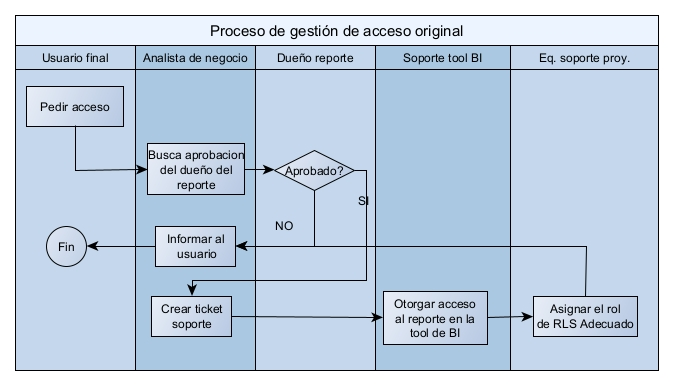
\includegraphics[width=15cm]{Workflow-aprobacion-original.jpg}
%\caption{proceso Original}
\end{tabular}

El nuevo proceso resultante, quita del medio todos los elementos de "complejidad accidental", dejando simplemente a los únicos dos roles, que son relevantes, el "End User" que es el usuario final quien solicita el acceso al reporte y el "Report Owner" que es quien determina si la solicitud corresponde o no y puede actuar en consecuencia.

EL proceso resultante de la simplificación e integración del portal conlas herramientas de visualización y también del RLS (en caso de ser necesario), se describe a continuación:

\begin{tabular}{l}
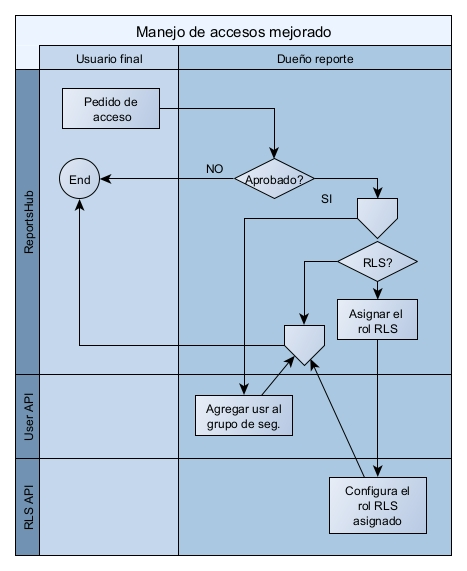
\includegraphics[width=10cm]{Workflow-aprobacion-mejorado.jpg}
%\caption{Proceso simplificado}
\end{tabular}

